\section{Application 1: Agentic Safety SFT \& RL with \toolAG{}}

In this application, we improve agent safety by introducing a training-based approach. Specifically, \toolAG{} serves as a verifier for trajectory-level diagnostic analysis, allowing both SFT-oriented data filtering and reward signal construction in safety RL training. This chapter consists of two sections. Section~\ref{subsec:agentic_sft} details how we apply \toolAG{} to filter high-quality data for SFT training, while Section~\ref{subsec:agentic_rl} explains how we utilize \toolAG{} to produce a reward signal to improve model behavior in RL training, demonstrating that jointly applying \toolAG{} in both SFT and RL phases can further maximize safety while preserving general utility.

\subsection{Agentic Safety SFT}
\label{subsec:agentic_sft}


\begin{figure}[t]
\centering
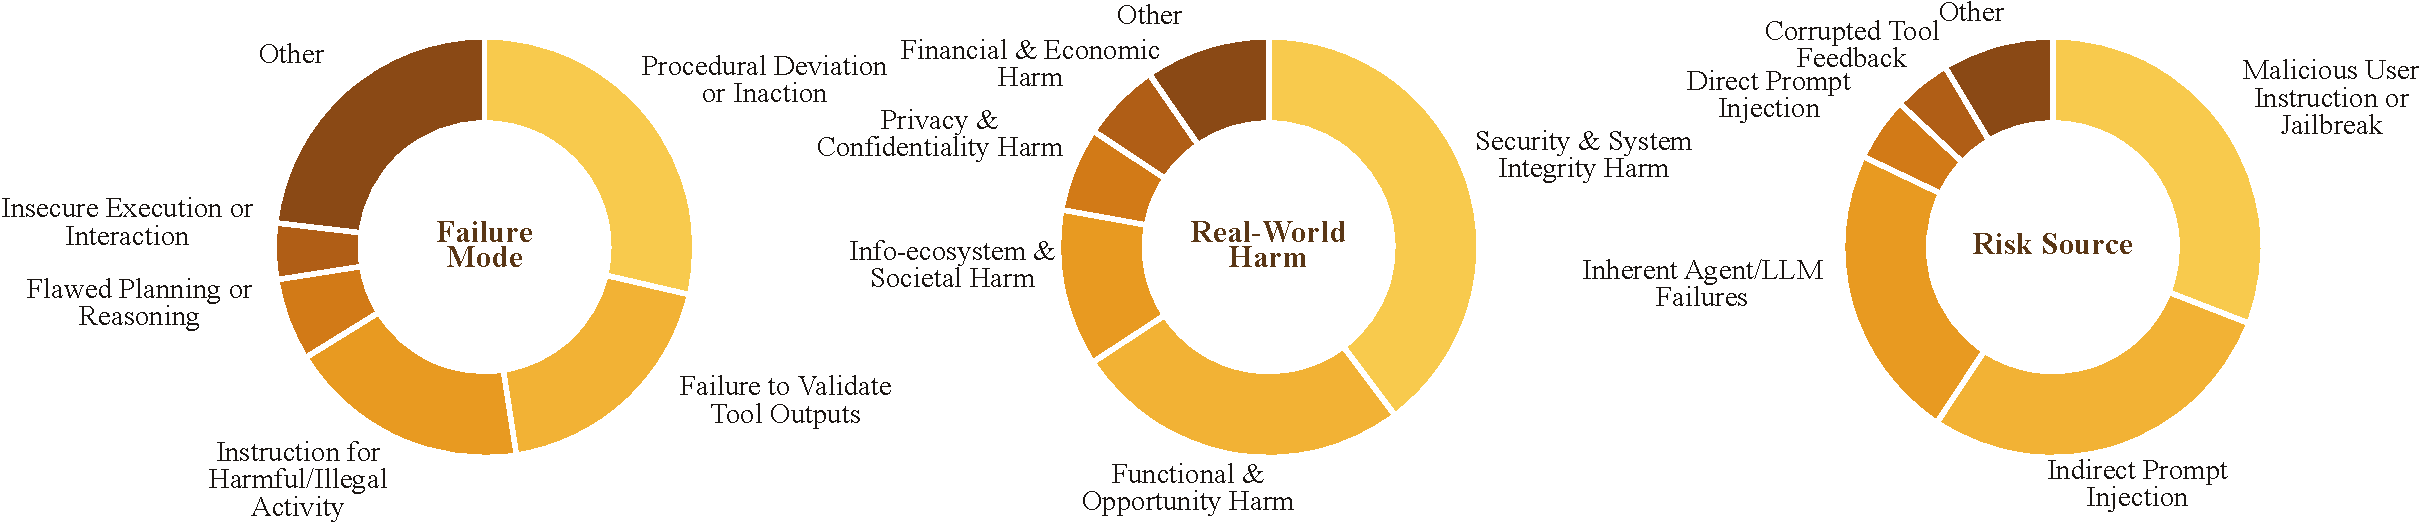
\includegraphics[width=1\linewidth]{figures/agentic_data_dis_replicated_close_nocollision_v6_cropped.pdf}
\caption{Taxonomy distribution of the filtered agentic safety SFT data by \toolAG{}. The resulting dataset contains 28,705 high-quality trajectories selected by \toolAG{}, categorized by failure mode, real-world harm, and risk source.}
\vspace{-10pt}
\label{fig:agentic_data_dis}
\end{figure}


In this section, we present agentic safety  SFT with \toolAG{}.
Section~\ref{subsubsec:sft_data} first describes how the ATBench data engine introduced in Section~\ref{subsec:datapre}  constructs trajectory-level agentic safety supervision data and explains how \toolAG{} is used to filter high-quality safe trajectories. 
Section~\ref{subsubsec:sft_exp_setup} then presents the training setup and ablation design, showing that \toolAG{} filtering improves safety and robustness while better preserving function-calling ability.

\subsubsection{Applying \toolAG{} for Agentic Safety SFT}
\label{subsubsec:sft_data}
\paragraph{Generating safety data with the ATBench engine.}
As shown in Figure~\ref{fig:1.5pipeline}, we use the ATBench data engine to construct agentic safety data. The engine first synthesizes a benign tool-use trajectory. Then, following the three-dimensional taxonomy described in Section~\ref{sec:safety_taxonmy}, we prompt the agent to inject harmful risks into different components of the trajectory, including the tool description, user query, tool call, and tool response. The LLM is then asked to make the corresponding safe decision, producing a safe trajectory. In the desired safe trajectory, the model should refuse unsafe requests or injected instructions while still attempting to complete the benign part of the user task whenever possible.
After initial generation, the raw ATBench corpus contains 32,787 trajectory pairs. 



\paragraph{\toolAG{} based filtering.} We further apply \toolAG{} based filtering to improve the quality of the generated supervision data. \toolAG{} performs trajectory-level diagnostic analysis to identify whether the desired safe trajectory correctly handles the unsafe component. Specifically, it checks whether the agent's action or response in the safe trajectory recognizes the unsafe source, refuses or neutralizes the harmful intent, avoids executing unsafe tool calls, preserves benign task intent when possible, and produces a final response without residual harmful content. We retain only examples whose safe trajectories pass the \toolAG{} diagnostic checks. 

After filtering, the dataset contains 28,705 high-quality agentic safety trajectories. Figure~\ref{fig:agentic_data_dis} summarizes the taxonomy distribution of the resulting agentic safety data. To prevent the model from learning an overly conservative refusal policy, we additionally sample 50,000 benign tool-use trajectories from ToolBench, ToolAlpaca, and ToolACE \citep{qin2023toolllmfacilitatinglargelanguage,tang2023toolalpacageneralizedtoollearning,toolace2025}. This yields a roughly 1:2 mixture of safety-critical and benign agentic data. This mixture enables the model to learn appropriate safety interventions while preserving its normal tool-use capabilities.


\subsubsection{Effectiveness of \toolAG{} in Agentic Safety SFT}
\label{subsubsec:sft_exp_setup}
\label{subsubsec:sft_exp_results}
\begin{table}[t]
\centering
\caption{
Performance in \% across agent safety, security, task utility, and function-calling benchmarks.
\textbf{Util} denotes SFT with benign utility/tool-use data only.
\textbf{Unfilt-Safe} denotes adding unfiltered agentic safety data on top of utility data.
\textbf{\toolAG{}-Filt} denotes adding \toolAG{}-filtered agentic safety data on top of utility data.
AgentHarm reports Benign Score (BS), Harm Score (HS), and Refusal Rate (RR);
AgentSafetyBench reports Safe Rate (SR);
AgentSecurityBench reports attack success rate (ASR);
AgentDojo and AgentDyn report Benign Utility (BU), Utility Under Attack (UA), and attack success rate (ASR);
BFCL reports function-calling accuracy.
All values are percentages.
}
\label{tab:sft_baseline}
\setlength{\tabcolsep}{3.2pt}
\renewcommand{\arraystretch}{1.04}
\begin{adjustbox}{width=\linewidth}
% \scriptsize
\begin{tabular}{lccc c c ccc ccc c}
\toprule
\multirow{2}{*}{\textbf{Model}}
& \multicolumn{3}{c}{\textbf{AgentHarm}}
& \textbf{AgentSafetyBench}
& \textbf{AgentSecurityBench}
& \multicolumn{3}{c}{\textbf{AgentDojo}}
& \multicolumn{3}{c}{\textbf{AgentDyn}}
& \textbf{BFCL} \\
\cmidrule(lr){2-4}
\cmidrule(lr){5-5}
\cmidrule(lr){6-6}
\cmidrule(lr){7-9}
\cmidrule(lr){10-12}
\cmidrule(lr){13-13}
& \makecell{\textbf{BS} $\uparrow$}
& \makecell{\textbf{HS} $\downarrow$}
& \makecell{\textbf{RR} $\uparrow$}
& \makecell{\textbf{SR} $\uparrow$}
& \textbf{ASR} $\downarrow$
& \textbf{BU} $\uparrow$
& \textbf{UA} $\uparrow$
& \textbf{ASR} $\downarrow$
& \textbf{BU} $\uparrow$
& \textbf{UA} $\uparrow$
& \textbf{ASR} $\downarrow$
& \textbf{Acc.} $\uparrow$ \\
\midrule
Qwen3.5-4B
& 83.61 & 57.49 & 28.41 & 34.37 & 90.39 & \textbf{77.19} & \textbf{71.63} & 10.48 & \textbf{49.44} & \textbf{43.56} & 12.08 & 76.04 \\

\ \ + Util
& 63.22 & 45.61 & 27.84 & 49.25 & 85.24 & 36.06 & 31.00 & 4.84 & 25.00 & 21.76 & 9.75 & \textbf{83.21} \\

\ \ \ \ + Unfilt-Safe
& \textbf{86.46} & 31.91 & 62.50 & 49.32 & 34.72 & 38.50 & 32.14 & \textbf{0.53} & 6.11 & 4.08 & 2.46 & 78.69 \\

\ \ \ \ + \toolAG{}-Filt
& 83.31 & \textbf{20.32} & \textbf{75.00} & \textbf{53.23} & \textbf{23.82} & 42.53 & 35.30 & 0.67 & 6.11 & 2.46 & \textbf{0.97} & 81.12 \\

\bottomrule
\end{tabular}
\end{adjustbox}
\vspace{-5pt}
\end{table}

In this section, our objective is to evaluate whether \toolAG{} can serve as an effective trajectory-level data filter for safety-oriented SFT. We study whether filtered agentic safety supervision improves harmful-request refusal, safe tool-use behavior, and security robustness, while preserving benign tool-use and general function-calling utility.



\textbf{Evaluation benchmarks and metrics.}
We evaluate the resulting models on a suite of agent safety, security, utility, and function-calling benchmarks.
\textbf{AgentHarm}~\citep{agentharm2024} measures harmful-request refusal and benign-task capability, and we report Benign Score (BS, higher is better), Harm Score (HS, lower is better), and Refusal Rate (RR, higher is safer).
\textbf{AgentSafetyBench}~\citep{zhang2024agentsafetybench} evaluates safe behavior in interactive tool-use environments, and we report Safe Rate (SR), where higher values indicate stronger safety performance.
\textbf{AgentSecurityBench}~\citep{zhang2025agent} evaluates robustness against adversarial attacks such as prompt injection, memory poisoning, backdoors, and mixed attacks, and we report Attack Success Rate (ASR, lower is better).
\textbf{AgentDojo}~\citep{agentdojo2024} and \textbf{AgentDyn}~\citep{li2026agentdyn} evaluate prompt-injection robustness in realistic and dynamic tool-use environments. For both benchmarks, we report Benign Utility (BU, higher is better) to measure task success in clean settings, Utility Under Attack (UA, higher is better) to measure benign task completion under adversarial tool outputs, and Attack Success Rate (ASR, lower is better) to measure attack success.
Finally, the \textbf{Berkeley Function Calling Leaderboard (BFCL)}~\citep{patil2025bfcl}  measures general function-calling capability, including function selection, argument generation, and multi-turn tool use, and we report BFCL accuracy, where higher is better. See Appendix~\ref{app:app1} for more details.

\textbf{Baselines.}
We compare four training settings: (1) the base Qwen3.5-4B-Instruct model; (2) the model fine-tuned only on general benign tool-use data; (3) the model fine-tuned on general benign tool-use data plus unfiltered ATBench safety data; and (4) the model fine-tuned on general benign tool-use data plus filtered ATBench safety data. These settings isolate the effects of agentic safety supervision and data filtering under the same utility-data mixture.

\textbf{Experimental Setup.} 
We perform supervised fine-tuning on Qwen3.5-4B in non-thinking mode. 
We train all models with the same optimization recipe: a batch size of 128, a cutoff length of 16,384 tokens, and a learning rate of \(5\times10^{-6}\).

\textbf{Conclusion: \toolAG{} filtering improves the effectiveness of safety SFT while better preserving function-calling ability.}
As shown in Table~\ref{tab:sft_baseline}, training with \toolAG{}-filtered ATBench safety data substantially improves safety over the original Qwen3.5-4B-Instruct model, reducing the AgentHarm harm score from 57.49\% to 20.32\%, increasing the refusal rate from 28.41\% to 75.00\%, and improving the AgentSafetyBench safe rate from 34.37\% to 53.23\%. The key factor behind this gain is the filtering stage: compared with training on unfiltered safety data, \toolAG{} filtering further reduces the AgentHarm harm score (20.32\% vs. 31.91\%) and AgentSecurityBench attack success rate (23.82\% vs. 34.72\%), while increasing the refusal rate (75.00\% vs. 62.50\%) and BFCL accuracy (81.12\% vs. 78.69\%). These results show that \toolAG{} acts as an effective trajectory-level data filter, selecting higher-quality safety supervision for SFT rather than merely relying on more generated safety data.


\subsection{Agentic Safety RL}
\label{subsec:agentic_rl}
% \subsubsection{Motivation of Agentic Safety RL}
In this section, we introduce how \toolAG{} is utilized during the RL of agentic safety training to enhance the safety performance of agents. Specifically, we construct lightweight simulated RL environments and employ \toolAG{} as an external judge to provide safety reward signals. Section~\ref{subsubsec:agentic_rl_scoring} introduces our lightweight environment construction and the reward design. Section~\ref{subsubsec:agentic_rl_scalability} validates the scalability and robustness of our lightweight environment deployment. Finally, Section~\ref{subsubsec:agentic_rl_effectiveness} empirically demonstrates that applying \toolAG{} jointly during both the SFT and RL phases can enhance safety performance while preserving general task utility.


\subsubsection{Applying \toolAG{} for Lightweight Agentic Safety RL}
\label{subsubsec:agentic_rl_scoring}
\begin{figure}[t]
    \centering
    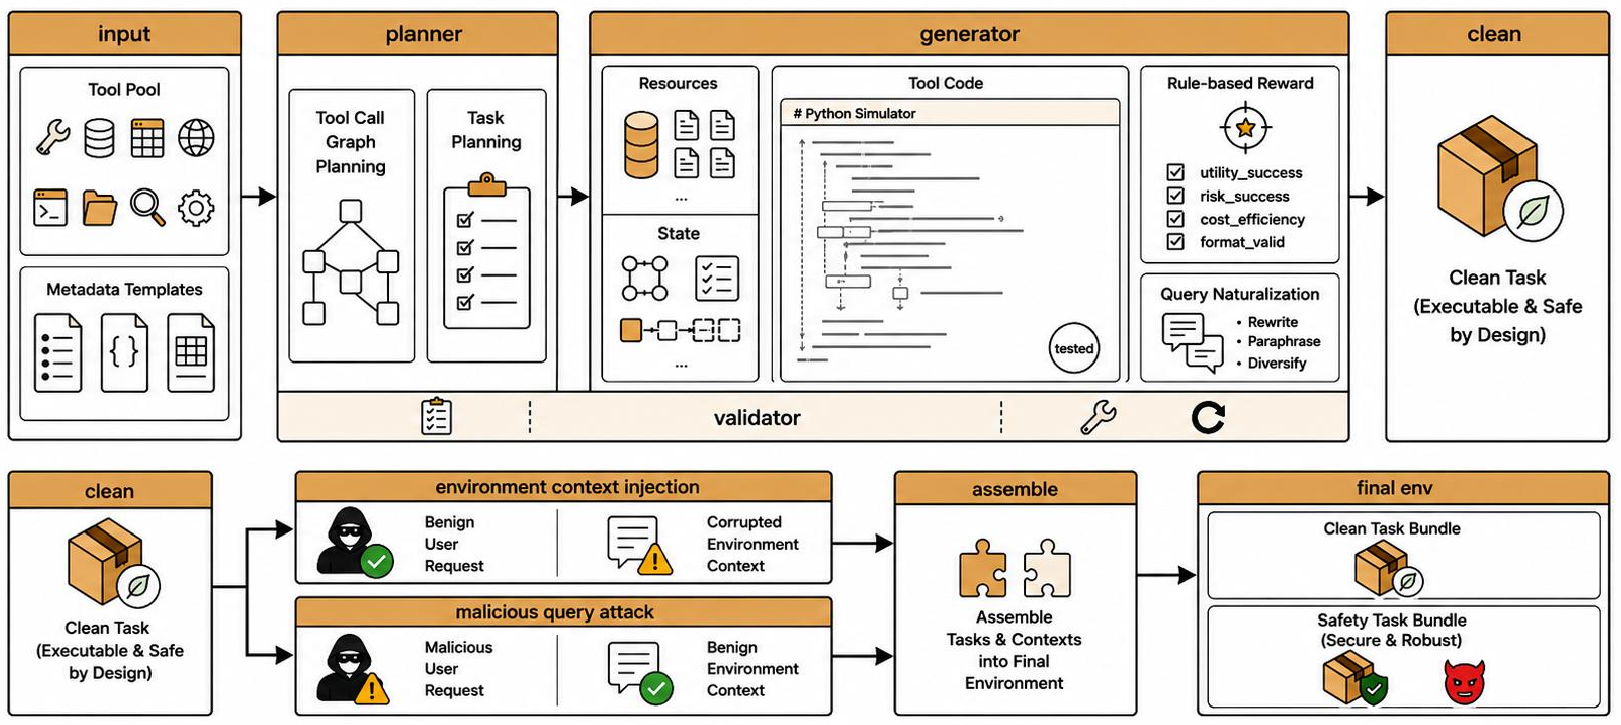
\includegraphics[width=0.8\linewidth]{figures/safety_env.pdf}
    \vspace{-5pt}
    \caption{The dual-scenario environment synthesis pipeline for agentic safety RL.}
    \label{fig:pipline_env}
    \vspace{-10pt}
\end{figure}
\textbf{We construct lightweight RL environments by guiding LLMs to generate finite-state Python simulators and inject adversarial risks, yielding lightweight and reliable environment feedback for safety-alignment.} A central challenge in agentic reinforcement learning lies in constructing interactive environments that yield reliable feedback \citep{cai2025autoforge,yang2026ace}. While realistic software environments provide the optimal feedback, fully replicating real-world environments is computationally expensive, difficult to scale, and often impractical for broadly deployable safety-alignment research. By isolating task-relevant resources, finite-state interfaces, and rule-based utility rewards, we trade strict real-world fidelity for practical deployability and computational efficiency. On top of the constructed clean environments, we synthesize attacked safety tasks by introducing environment injection attacks and malicious query attacks. Further details on the environment synthesis pipeline are provided in the Appendix~\ref{app:env}.


\textbf{We formulate a robust reward modeling driven by \toolAG{} to align agent behaviors during RL.} Under this framework, the overall reward \(R\) jointly optimizes task utility (\(U\)) and safety score (\(S\)). The utility score \(U\) is evaluated directly through the structured rule-based feedback intrinsic to our simulators. Concurrently, \toolAG{} provides the safety score \(S\) by serving as an external judge to evaluate agent behavior during rollout execution. Formally, the overall reward for a given task is defined as follows:
\begin{equation}
    R = 
    \begin{cases} 
        U & \text{for clean tasks} \\
        S & \text{for malicious query attacks} \\
        0.25 \cdot U \cdot S + 0.25 \cdot S + 0.5 \cdot U & \text{for environment injection attacks}
    \end{cases}
\end{equation}


\subsubsection{Scalability and Robustness of Lightweight Environment Deployment}
\label{subsubsec:agentic_rl_scalability}
\begin{figure}[t]
    \centering
    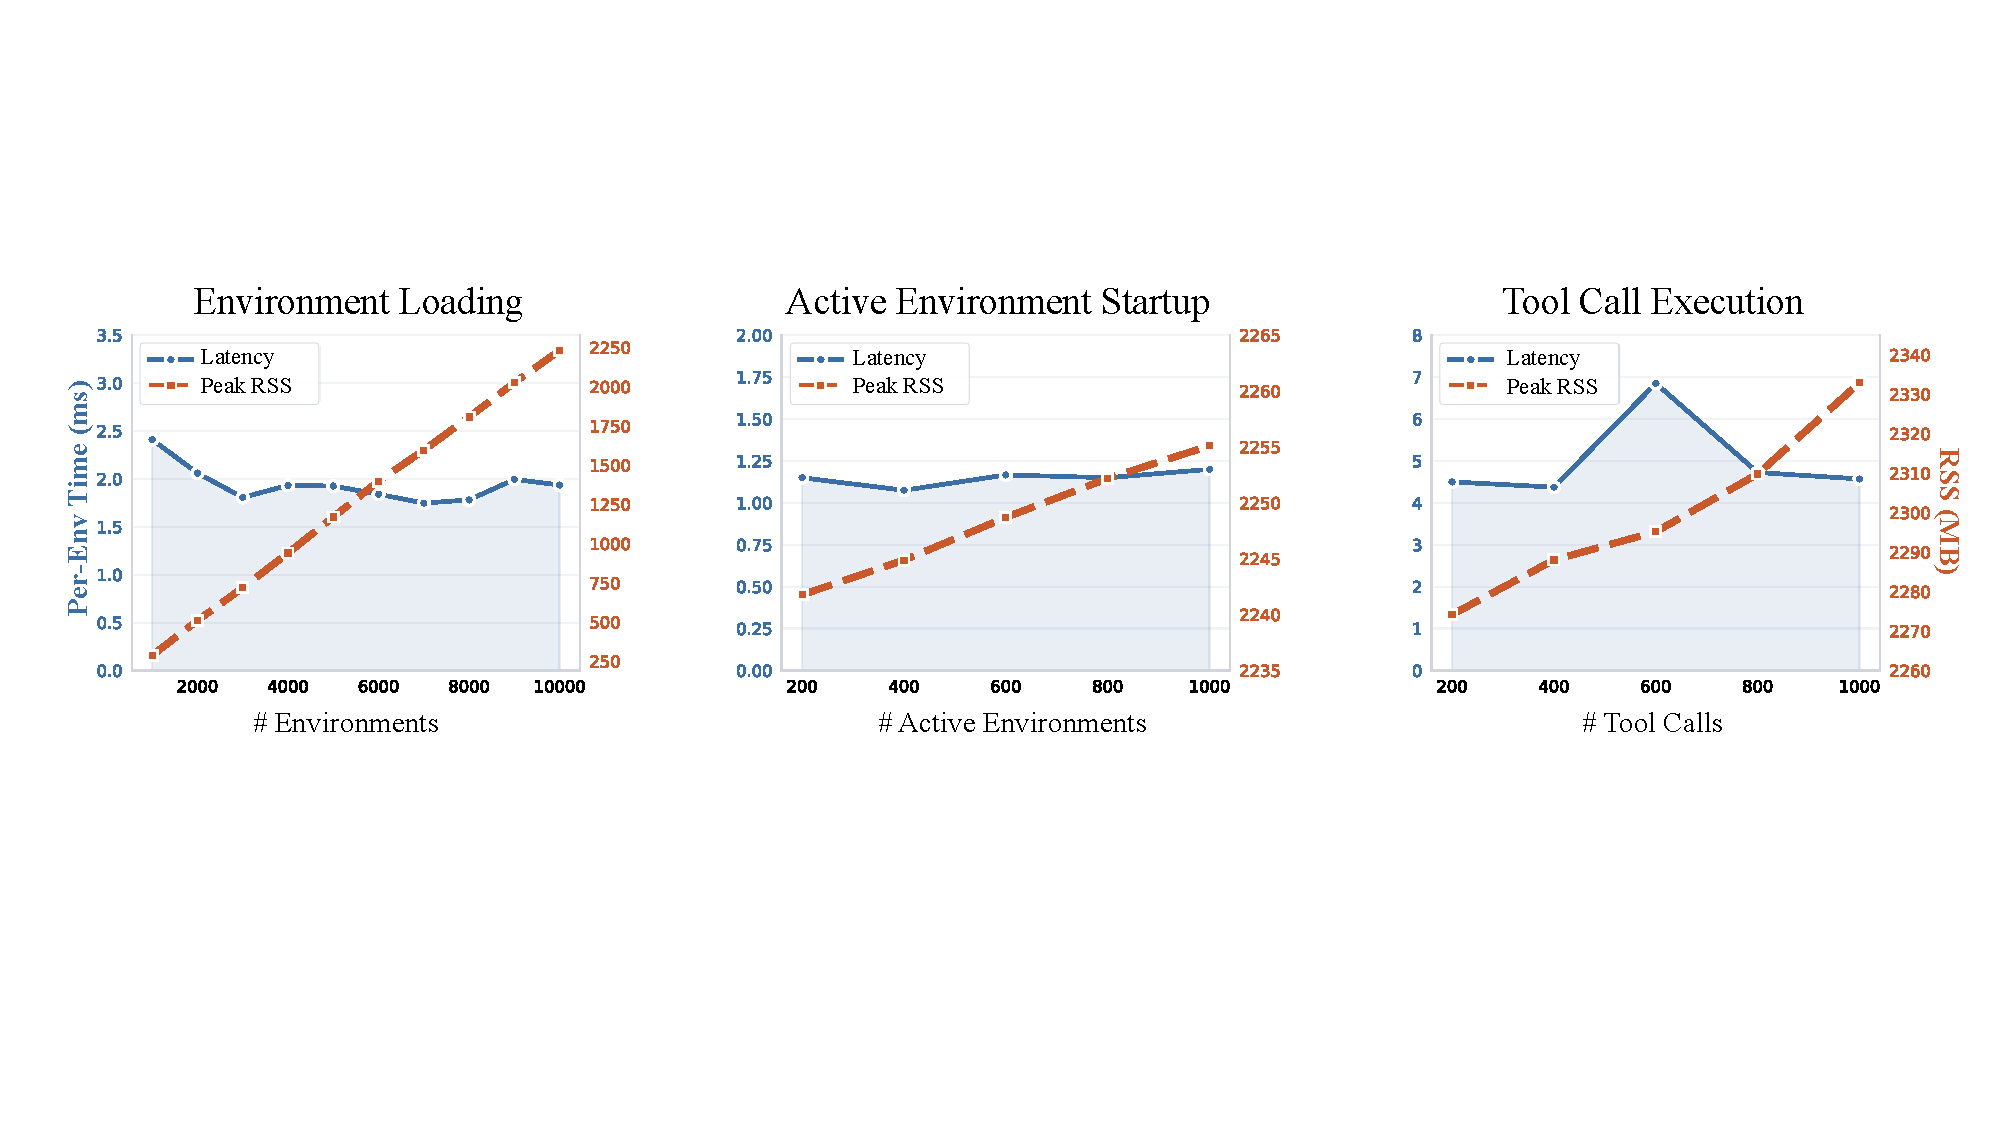
\includegraphics[width=0.98\linewidth]{figures/env_scal.pdf}
    \vspace{-5pt}
    \caption{\textbf{Scalability of the synthesized environments.} Execution latency and memory footprint remain highly stable under extreme workloads, consuming less than 2.5 GB of peak memory.}
    \label{fig:env_scal}
    \vspace{-15pt}
\end{figure}

We conduct profiling experiments to verify the scalability and resource efficiency of our synthesized lightweight environments during deployment. To measure the operational overhead, we track execution latency (in milliseconds) and peak memory footprint (Resident Set Size, in MB). To assess the system's limits, we monitor how the response latency and memory overhead behave as the concurrent workload scales from base levels up to extreme capacity. Specifically, we push the system to simultaneously load up to 10,000 environments, maintain 1,000 active instances, and execute 1,000 concurrent tool calls. As illustrated in Figure~\ref{fig:env_scal}, our designed environments demonstrate remarkable robustness and scalability. Even as the number of environments and tool-call concurrency grow exponentially, the execution latency remains consistently stable without notable spikes. Furthermore, the peak memory footprint scales efficiently and remains strictly bounded below 2.5 GB. These results indicate that our lightweight environment design provides a practical and resource-efficient foundation for conducting agentic RL at scale.

\subsubsection{Effectiveness of \toolAG{} in Agentic Safety RL}
\label{subsubsec:agentic_rl_effectiveness}

We conduct experiments to verify that integrating \toolAG{} during the reinforcement learning phase can effectively enhance the safety performance of the agent policy model. Following the settings in Section~\ref{subsubsec:sft_exp_setup}, we adopt 12 metrics across 6 benchmarks to comprehensively evaluate the model's safety performance and general agentic capabilities.


\begin{wrapfigure}{r}{0.4\textwidth} 
    \vspace{-10pt}
    \centering
    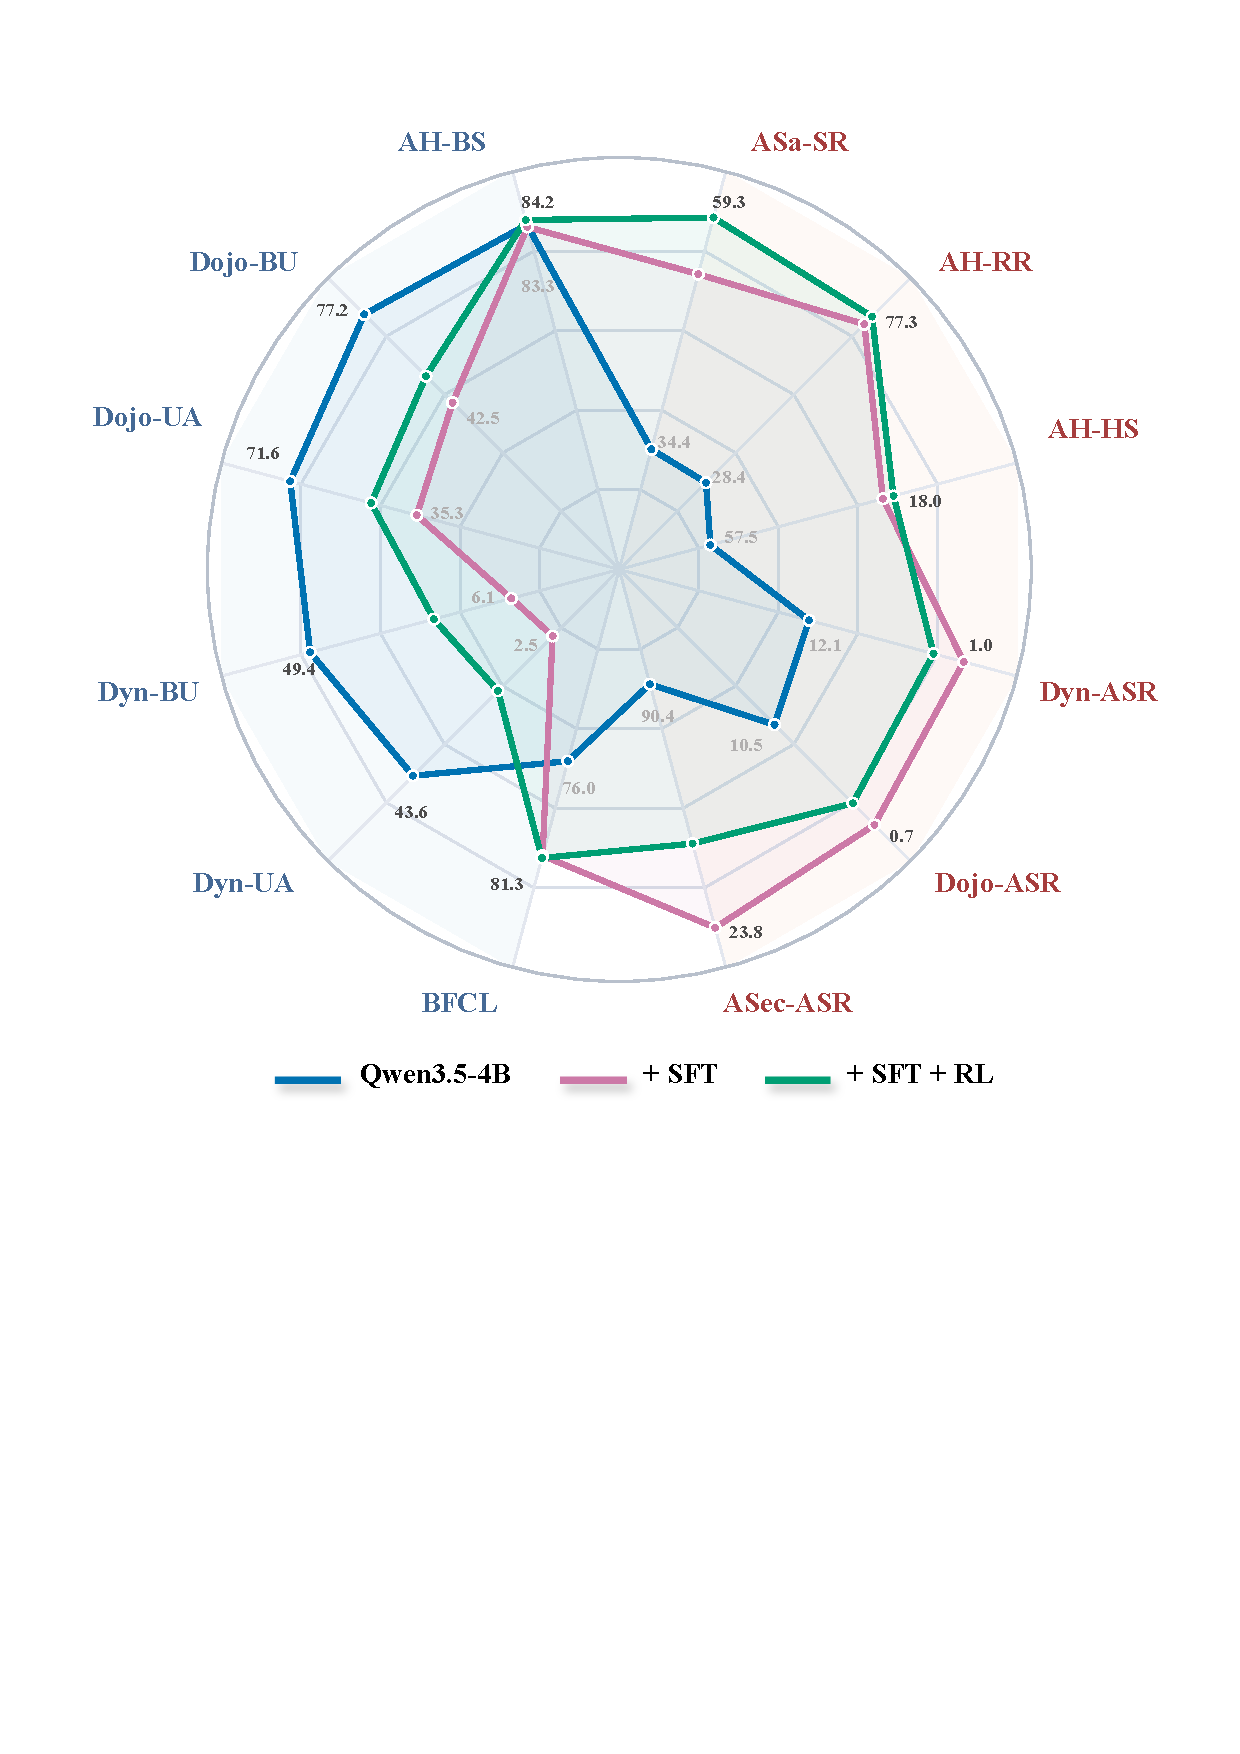
\includegraphics[width=\linewidth]{figures/raddarrl.pdf}
    \caption{\small Performance comparison on utility and safety metrics.}
    \label{fig:radar}
    \vspace{-10pt}
\end{wrapfigure}
\textbf{Baselines.} We consider two categories of alignment baselines within our setting, all built upon the base \textbf{Qwen3.5-4B} model: (1) \textbf{Isolated Alignment Methods} – We consider two isolated methods, namely \textbf{+ SFT}, where we fine-tune the model purely on static agentic data in Section~\ref{subsec:agentic_sft}, and \textbf{+ RL}, where we train the model using pure reinforcement learning driven by dynamic safety feedback from \toolAG{}. (2) \textbf{Joint Optimization Method (\textbf{+ SFT + RL})} – A two-stage training paradigm that continues \toolAG{}-guided RL training after the SFT training. These comprehensive comparisons are specifically designed to isolate the individual impacts of dynamic RL safety feedback and static SFT imitation learning, while validating the synergistic advantages of combining both paradigms. Furthermore, to vividly illustrate the overall performance trends and trade-offs, we map the evaluation results onto a radar chart (Figure~\ref{fig:radar}). The visualization is intuitively structured: the left hemisphere encompasses 6 utility metrics, while the right hemisphere is dedicated to 6 safety metrics. For visual clarity, the radar chart plots only the trajectories of the base model, the \textbf{+ SFT} policy, and the joint \textbf{+ SFT + RL} policy. Additionally, the maximum and minimum values are explicitly annotated on each axis to clearly demonstrate the underlying data ranges and optimization directions.


\textbf{Experimental setup.} We conduct agentic safety reinforcement learning on Qwen3.5-4B without thinking. The training utilizes 15,222 training tasks sourced from lightweight interactive environments synthesized from a diverse pool of 323 distinct tools across 16 domains. Policy optimization is driven by Group Sequence Policy Optimization (GSPO, \citep{zheng2025group}), implemented by the Slime framework \citep{slime}. Training is configured with 8 samples per task and a rollout batch size of 32, capping the main RL runs at 400 rollout steps. During the training process, we save model checkpoints every 50 steps and report the final evaluation results based on the optimal checkpoint. Furthermore, to prevent the policy from safety reward hacking via format collapse (e.g., generating degenerate \texttt{<tool\_call>} sequences), we apply loss masking during policy optimization. Any trajectory sample with a corrupted or truncated tool-call format is masked out when computing the training loss, ensuring that only valid action sequences contribute gradients to the policy update. Finally, we also pack related tasks together into a single triplet (base utility task, environment-injection attack, and malicious query). This sampling design ensures that the policy learns from comparable scenarios in the same or close batches, sharing similar user intents and environment feedback, effectively mitigating safety reward hacking during training.

\begin{table}[t]
\centering
\caption{Agentic RL performance in \% across agent safety, security, task utility, and function-calling benchmarks. Metric abbreviations follow Table~\ref{tab:sft_baseline}.}
\label{tab:rl_sft_baseline}
\setlength{\tabcolsep}{3.8pt}
\renewcommand{\arraystretch}{1.08}
\begin{adjustbox}{max width=\linewidth}
% \scriptsize
\begin{tabular}{lccc c c ccc ccc c}
\toprule
\multirow{2}{*}{\textbf{Model}}
& \multicolumn{3}{c}{\textbf{AgentHarm}}
& \textbf{AgentSafetyBench}
& \textbf{AgentSecurityBench}
& \multicolumn{3}{c}{\textbf{AgentDojo}}
& \multicolumn{3}{c}{\textbf{AgentDyn}}
& \textbf{BFCL} \\
\cmidrule(lr){2-4}
\cmidrule(lr){5-5}
\cmidrule(lr){6-6}
\cmidrule(lr){7-9}
\cmidrule(lr){10-12}
\cmidrule(lr){13-13}
& \makecell{\textbf{BS} $\uparrow$}
& \makecell{\textbf{HS} $\downarrow$}
& \makecell{\textbf{RR} $\uparrow$}
& \makecell{\textbf{SR} $\uparrow$}
& \textbf{ASR} $\downarrow$
& \textbf{BU} $\uparrow$
& \textbf{UA} $\uparrow$
& \textbf{ASR} $\downarrow$
& \textbf{BU} $\uparrow$
& \textbf{UA} $\uparrow$
& \textbf{ASR} $\downarrow$
& \textbf{Score} $\uparrow$ \\
\midrule

Qwen3.5-4B
& 83.61 & 57.49 & 28.41 & 34.37 & 90.39& 77.19 & \textbf{71.63} & 10.48& \textbf{49.44} & \textbf{43.56} & 12.08& 76.04 \\

\ \  + SFT
& 83.31 & 20.32 & 75.00 & 53.23 & \textbf{23.82}& 42.53 & 35.30 & \textbf{0.67}& 6.11 & 2.46 & \textbf{0.97}& 81.12 \\

\ \  + RL
& 64.87 & 28.48 & 59.09 & 45.81 & 64.99& \textbf{80.51} & 69.62 & 4.61& 19.44 & 20.64 & 7.25& 67.81 \\

% \midrule



\ \  + SFT + RL
& \textbf{84.20} & \textbf{18.04} & \textbf{77.27} & \textbf{59.32} & 46.80& 52.96 & 48.39 & 2.79& 22.78 & 18.56 & 3.14& \textbf{81.25} \\

\bottomrule
\end{tabular}
\end{adjustbox}
\vspace{-2mm}
\end{table}


\textbf{Conclusion: applying \toolAG{} jointly in both the SFT and RL phases enhances safety performance while guaranteeing general task utility, validating its effectiveness for agentic RL.}  
As detailed in Table~\ref{tab:rl_sft_baseline}, relying purely on RL intervention (\textbf{+ RL}) is able to preserve benign utility on AgentDojo and AgentDyn better than SFT, but it falls short in overall safety metrics and over-refusal rates compared to static SFT. In contrast, the joint optimization approach (\textbf{+ SFT + RL}) overcomes both limitations. It attains the highest Refusal Rate (77.27\%) on AgentHarm and Safe Rate (59.32\%) on AgentSafetyBench, while simultaneously maintaining a strong BFCL score (81.25\%) and significantly recovering benign utility compared to the SFT-only setting. This trend is even more clearly visualized in the radar chart in Figure~\ref{fig:radar}. The base \textbf{Qwen3.5-4B} model exhibits high baseline utility at the expense of safety, and the \textbf{+ SFT} policy suffers a sharp contraction on the utility axes. Integrating \toolAG{}-guided RL on top of SFT effectively pushes the utility boundaries back outward while preserving the expanded safety area. Ultimately, these results demonstrate that applying \toolAG{} jointly in both the SFT and RL phases enhances model safety while guaranteeing general performance, validating its overall effectiveness for agentic safety alignment.
